\documentclass{article}

\usepackage[final]{nips_2017}

\usepackage[utf8]{inputenc} % allow utf-8 input
\usepackage[T1]{fontenc}    % use 8-bit T1 fonts
\usepackage{hyperref}       % hyperlinks
\usepackage{url}            % simple URL typesetting
\usepackage{booktabs}       % professional-quality tables
\usepackage{amsfonts}       % blackboard math symbols
\usepackage{nicefrac}       % compact symbols for 1/2, etc.
\usepackage{microtype}      % microtypography
\usepackage{graphicx}
\usepackage{amsmath}
\usepackage{amssymb}
\usepackage{listings}
\usepackage{courier}
\lstset{basicstyle=\ttfamily\footnotesize,breaklines=true}
\title{CSE 253 Programming Assignment 2 -- Multilayers Back-propagation Neural Networks}

\author{
  Fanjin Zeng \\
  Computer Science and Engineering\\
  University of Califorina, San Diego\\
  \texttt{f1zeng@ucsd.edu} \\
   \And
   Xinyue Ou \\
   Computer Science and Engineering\\
   University of Califorina, San Diego \\
   \texttt{x1ou@ucsd.edu} \\
}

\begin{document}

\maketitle
\begin{abstract}
	
\end{abstract}
\section{Classification}
\subsection{}
\subsection{}
\subsection{}
\subsection{}

\newpage
\section{Adding the "Tricks of the Trade"}
\subsection{}
\subsection{}
\subsection{Weight Initialization}
Our code actually starts with this trick. It initializes the weights to be a normal distribution with 0 mean and unit deviation. What's different is that we employ fan-in factor this time. Before the test accuracy is 0.9656 and after that it is 0.9679. It improves a little bit, but not help that much.
\subsection{Momentum}
Momentum is a good way to speed up the training. We compare the difference between the original gradient descent, the one with momentum and the one with Adam optimizer.

\begin{figure}[h]
	\begin{minipage}{0.3\textwidth}
	\centering
	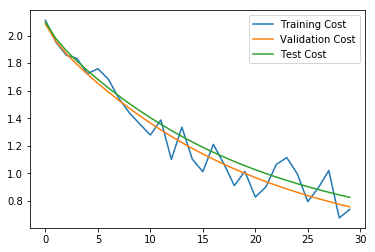
\includegraphics[width=\textwidth]{pics/loss_original.png}
	\caption{Loss function over training epoch. Original gradient descent}
	\end{minipage}\hfill
	\begin{minipage}{0.3\textwidth}
	\centering
	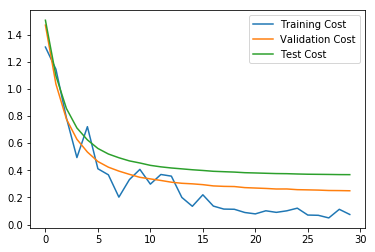
\includegraphics[width=\textwidth]{pics/loss_momentum.png}
	\caption{Loss function over training epoch. Gradient descent with momentum}
	\end{minipage}\hfill
	\begin{minipage}{0.3\textwidth}
	\centering
	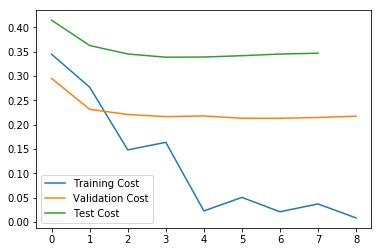
\includegraphics[width=\textwidth]{pics/loss_adam.png}
	\caption{Loss function over training epoch. Adam optimizer}
	\end{minipage}
\end{figure}

The original gradient descent takes 300 epochs of training and arrives at 0.73 loss at the 300th epoch. The gradient descent with momentum also reaches 0.73 loss, but it arrives at the value that is very close to it at the 200th epoch. The Adam optimizer is even faster, it reaches 0.03 at the 80th epoch, and then early stops.


\newpage
\section{Experiment with Network Topology}
\subsection{Double Hidden Units}
When doubling the number of hidden units, i.e., training with 128 neural in the hidden layers, we achieve a test rate of 96.5\%, which is not that different from the one with 64 layers. The tricky part is, when we keep increases the number of hidden layer, the accuracy actually went up quite significantly, reaching more than 98\%.
\begin{figure}[h]
\centering
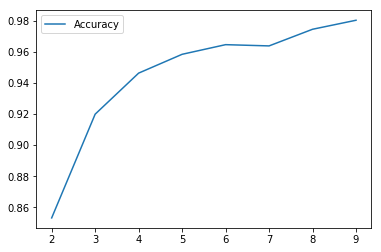
\includegraphics[width=0.5\textwidth]{pics/acc_hidden.png}
\caption{Testing accuracy vs hidden unit number in log scale}
\end{figure}
If the number of the hidden units is too small, the accuracy goes down, but higher number of hidden units significantly increases the training period.

\subsection{Double Hidden Layers}
We use a network with first layer having 48 units and the second one having 16. The testing accuracy of it is 96.21\%.
\begin{figure}[h]
	\begin{minipage}{0.48\textwidth}
	\centering
	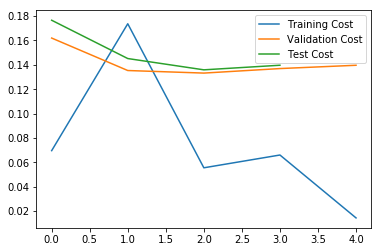
\includegraphics[width=\textwidth]{pics/loss_double.png}
	\caption{Loss function over training epoch, with first hidden layer having 48 units and the second having 16}
	\end{minipage}\hfill
	\begin{minipage}{0.48\textwidth}
	\centering
	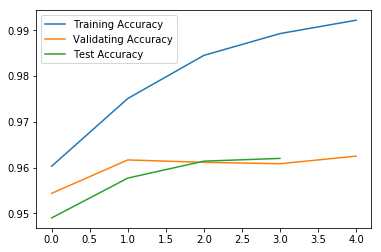
\includegraphics[width=\textwidth]{pics/acc_double.png}
	\caption{Loss function over training epoch, with first hidden layer having 48 units and the second having 16}
	\end{minipage}
\end{figure}

\subsection{Extra: Adam Optimizer}
We use adam optimizer for updating parameters, which usually helps to get faster convergence. The result has been mentioned above.  
\end{document}